\documentclass[ 12pt, a4paper]{article}
% Use the option doublespacing or reviewcopy to obtain double line spacing
% \documentclass[doublespacing]{elsart}

\usepackage[utf8]{inputenc}
\usepackage[backend = biber, maxcitenames=2,uniquelist=minyear]{biblatex}

\AtEveryBibitem{\clearfield{number}}
\AtEveryBibitem{\clearfield{doi}}
\AtEveryBibitem{\clearfield{url}}
\AtEveryBibitem{\clearfield{issn}}
\AtEveryBibitem{\clearfield{isbn}}

\addbibresource{references.bib}

\usepackage{color,graphicx,tikz}
\usetikzlibrary{positioning,arrows}
% The amssymb package provides various useful mathematical symbols
\usepackage{mathtools,amssymb,amsmath,mathdots}
\usepackage[mathscr]{eucal} %just for the font \mathscr
\usepackage{setspace}
\usepackage{hyperref}

\usepackage{tikz}

\renewcommand{\vec}[1]{\boldsymbol{#1}}
\renewcommand{\thefootnote}{\fnsymbol{footnote}}

\newcommand{\inc}{\mathrm{inc}}
\newcommand{\scat}{\mathrm{s}}

\newcommand{\ii}{\mathrm{i}}
\newcommand{\ee}{\mathrm{e}}

\renewcommand{\vec}[1]{\boldsymbol{#1}}


\begin{document}

\title{Acoustic multiple scattering}
\author{
Artur L. Gower$^{a}$,\\
\footnotesize{$^{a}$ School of Mathematics, University of Manchester, Oxford Road, Manchester, M13 9PL,UK}
}
\date{\today}
\maketitle

\begin{abstract}
Here we show and deduce the T-matrix and multiple scattering for acoustics. Before reading this document, it may be helpful to read the general multiple scattering formulation shown in \href{multiplescattering.pdf}{multiplescattering.pdf}.
\end{abstract}

\noindent
{\textit{Keywords:} Multiple scattering, T-matrix, Scattering matrix}

\section{2D acoustics}
Much of the notation is define in \href{multiplescattering.pdf}{multiplescattering.pdf}. For the 2D acoustics some good references are \parencite{ganesh_far-field_2010,ganesh_algorithm_2017}.

For 2D acoustics we have that
\begin{align}
  & \mathrm u_{n}(k\rv) = J_{n}(k r) \ee^{\ii n \theta},
  \\
  & \mathrm v_{n}(k\rv)= H_{n}(k r) \ee^{\ii n \theta}.
\end{align}
When truncating up to some order $N$ we would sum over $n = -N, -N +1, \ldots, N-1, N$.


\subsection{Circular cylinder}
Let $\rho$ and $c$ be the background density and wavespeed, and let $\rho_j$, $c_j$ and radius $a_j$ be the mass density, wavespeed, and radius for a circular scatterer with density.

Let $u = \ui + \us$ be the total field outside the particle, and $\vi$ the total field inside the particle, then from the acoustic boundary conditions:
\[
u = \vi, \quad \frac{1}{\rho} \frac{\partial u}{\partial r} = \frac{1}{\rho_j} \frac{\partial \vi}{\partial r}, \quad \text{for} \;\; r = a_j,\
\]
we can deduce the T-matrix
\begin{equation}
  T_{nm} = - \delta_{nm} \frac{\gamma_j J_m' (k a_j) J_m (k_j a_j) - J_m (k a_j) J_m' (k_j a_j) }{\gamma_j H_m '(k a_j) J_m(k_j a_j) - H_m(k a_j) J_m '(k_j a_j)},
  \label{eqn:circular_t-matrix}
\end{equation}
where $\gamma_j = (\rho_j c_j)/(\rho c)$ and $k_j = \omega/c_j$.

We can also calculate the coefficients $b_n$ from
\begin{equation}
  b_n = \frac{f_n}{T_{nn} J_n(k_ja_j)}\left[ T_{nn} H_n(ka_j) + J_n(k a_j) \right]
\end{equation}



\subsection{Circular cylindrical capsule}

\begin{figure}[t]
\centering
  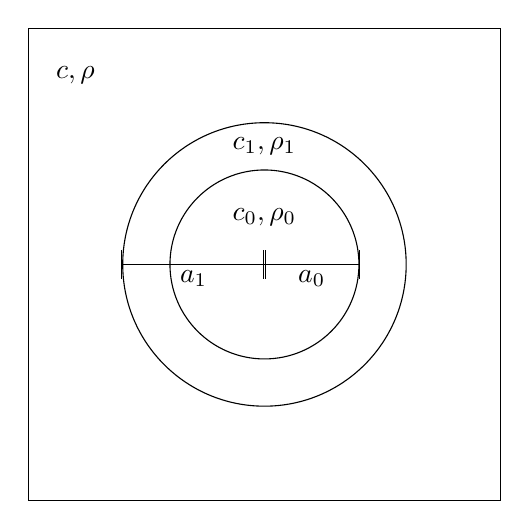
\begin{tikzpicture}[scale=0.6]
  % Outer box
  \draw (-5,-5) -- (5,-5) -- (5,5) -- (-5,5) -- (-5,-5);

  % Concentric circles
  \draw (0,0) circle (2);
  \draw (0,0) circle (3);

  % Line to show a_1
  \draw (-3.02, 0) -- (-0.02,0);
  \draw (-3.02, 0.3) -- (-3.02,-0.3);
  \draw (-0.02, 0.3) -- (-0.02,-0.3);
  \node at (-1.5,-0.3) { $a_1$ };

  % Line to show a_0
  \draw (2.02, 0) -- (0,0);
  \draw (2.02, 0.3) -- (2.02,-0.3);
  \draw (0.02, 0.3) -- (0.02,-0.3);
  \node at (1,-0.3) { $a_0$ };

  \node at (-4,4) { $c,\rho$ };
  \node at (0,1) { $c_0,\rho_0$ };
  \node at (0,2.5) { $c_1,\rho_1$ };

  \end{tikzpicture}

  \label{fig:capsule}
\end{figure}

\begin{align}
  & \psi^0 = \sum_{n=-\infty}^\infty g_n^0 J_{n}(k_0 r) \ee^{\ii n \theta},
  \\
  & \psi^1 = \sum_{n=-\infty}^\infty \left [ g_n^1 J_{n}(k_1 r) + f_n^1 H_{n}(k_1 r) \right ] \ee^{\ii n \theta}.
\end{align}
Applying the boundary conditions,
\begin{align}
  	& \psi^0 = \psi^1 \quad \text{and} \quad \frac{1}{\rho_0} \frac{\partial \psi^0}{\partial r} = \frac{1}{\rho_1} \frac{\partial \psi^1}{\partial r}, \quad \text{on} \;\; r = a_0,
    \label{eqn:inner_bc}
    \\
  	& \psi^1 = \psi^\scat + \psi^\inc \quad \text{and} \quad \frac{1}{\rho_1} \frac{\partial \psi^1}{\partial r} = \frac{1}{\rho} \frac{\partial (\psi^\scat + \psi^\inc)}{\partial r}, \quad \text{on} \;\; r = a_1.
    \label{eqn:outer_bc}
\end{align}
Solving these boundary conditions (see \href{capsule-boundary-conditions.nb}{capsule-boundary-conditions.nb}) leads to
\begin{multline}
  T_{nn} = - \frac{J_n(k a_1)}{H_n(k a_1)} - \frac{Y^n_{'}(k a_1, k a_1)}{H_n(ka_1)} \left[Y^n(k_1 a_1,k_1 a_0) J_n'(k_0 a_0) - q_0 J_n(k_0 a_0) Y^n_{'}(k_1 a_1,k_1 a_0) \right]
  \\ \times \big[
    J_n'(k_0 a_0)(q H_n(k a_1)Y^n_{'}(k_1 a_0,k_1 a_1) + H_n'(k a_1) Y^n(k_1 a_1,k_1 a_0))
    \\
    + q_0 J_n(k_0 a_0)(q H_n(k a_1)Y^n_{''}(k_1 a_1,k_1 a_0) - H_n'(k a_1) Y^n_{'}(k_1 a_1, k_1 a_0))
  \big]^{-1}.
\end{multline}
where $q = \rho c/(\rho_1 c_1)$, $q_0 = \rho_0 c_0/( \rho_1 c_1)$, and
\begin{align}
  & Y^n(x,y) = H_n(x) J_n(y) - H_n(y) J_n(x), \\
  & Y^n_{'}(x,y) = H_n(x) J_n'(y) - H_n'(y) J_n(x), \\
  & Y^n_{''}(x,y) = H_n'(x) J_n'(y) - H_n'(y) J_n'(x).
\end{align}

% Using~\eqref{eqn:inner_bc} we get
% \begin{align}
%   & g_n^0 J_{|n|}(k_0 a_0) = g_n^1 J_{|n|}(k_1 a_0) + a_n^0 H_{|n|}(k_1 a_0),
%   \\ \notag
%   & g_n^1 \left [ \frac{J_{|n|}'(k_0 a_1)}{\rho_0 c_0} \frac{J_{|n|}(k_1 a_0)}{J_{|n|}(k_0 a_0)} - \frac{J_{|n|}'(k_1 a_1)}{\rho_1 c_1} \right ] =
%   a_n^1 \left [ \frac{J_{|n|}'(k_0 a_1)}{\rho_0 c_0} \frac{H_{|n|}(k_1 a_0)}{J_{|n|}(k_0 a_0)} - \frac{H_{|n|}'(k_1 a_1)}{\rho_1 c_1} \right ].
% \end{align}
%
% \begin{gather}
%    g_n^1 J_{|n|}(k_1 a_1) + a_n^1 H_{|n|}(k_1 a_1) =  g_n J_{|n|}(k a_1) + a_n H_{|n|}(k a_1)
%    \\
%    g_n^1 \frac{1}{\rho_1 c_1} J_{|n|}'(k_1 a_1) + a_n^1 \frac{1}{\rho_1 c_1} H_{|n|}'(k_1 a_1)
%    =  g_n \frac{1}{\rho c} J_{|n|}'(k a_1) + a_n \frac{1}{\rho c} H_{|n|}'(k a_1)
% \end{gather}

\subsection{Multiple scattering in 2D}

Graf's addition theorem in two spatial dimensions:
\begin{align}
  & H_n(k R_\ell)\ee^{\ii n \Theta_\ell} =
  \sum_{m=-\infty}^\infty H_{n-m}(k R_{\ell j})\ee^{\ii(n-m)\Theta_{\ell j}} J_{m}(k R_j)\ee^{\ii m \Theta_j}, \;\;\text{for}\;\; R_j < R_{\ell j},
\label{eqn:Graf}
\end{align}
where $(R_{\ell j},\Theta_{\ell j})$ are the polar coordinates of $\vec r_j - \vec r_\ell$. The above is also valid if we swap $H_n$  for $J_n$, and swap $H_{n-m}$ for $J_{n-m}$.

Particle-$j$ scatters a field
\begin{equation}
  \label{eqn:outwaves}
  u_j = \sum_{n} f_n^j \mathrm u_{n}(k\rv - k \rv_j), \quad \text{for} \;\; |\rv - \rv_j| > a_j,
\end{equation}
% where $(R_j,\Theta_j)$ are the polar coordinates of $\vec r - \vec r_j$,
where $\vec r_j$ is the centre of particle $j$.

Let the incident wave, with coordinate system centred at $\vec r_j$, be
\begin{equation}
  \label{eqn:incident}
  \ui = \sum_{n} g_n^j \mathrm v_{n}(k\rv - k \rv_j),
\end{equation}
then the wave exciting particle-$j$ is
\begin{equation}
  \label{eqn:exciter}
  u_j^E = \sum_{n} F^n_j \mathrm v_{n}(k\rv - k \rv_j)
\end{equation}
where
\begin{equation}
  F_n^j = g_n^j + \sum_{\ell\not = j} \sum_{p=-\infty}^\infty f_p^\ell H_{p-m}(k R_{\ell j})\ee^{\ii(p-m)\Theta_{\ell j}}.
\end{equation}
Using the T-matrix of particle-$j$ we reach $f_n^j = \sum_m T_{nm}^j F_m^j$, which leads to
\begin{equation}
f_q^j  = \sum_{m} T_{qm}^j g_m^j + \sum_{\ell\not = j} \sum_{m,p=-\infty}^\infty f_p^\ell T_{qm}^j H_{p-m}(k R_{\ell j})\ee^{\ii(p-m)\Theta_{\ell j}}.
\label{eqn:As}
\end{equation}
The above simplifies if we substitute $f_q^j =  T_{qd}^j \alpha_d^j$, and then multiple across by $\{T_{qn}^j\}^{-1}$ and sum over $q$ to arrive at
% f_\ell^p = \alpha_\ell^d T^{dp}_\ell
% f_\ell^p = \alpha_\ell^d T^{dp}_\ell
\begin{equation}
\alpha_n^j = g_n^j + \sum_{\ell\not = j} \sum_{m,p=-\infty}^\infty  H_{p-n}(k R_{\ell j})\ee^{\ii(p - n)\Theta_{\ell j}} T_{pm}^\ell \alpha_m^\ell.
\label{eqn:As}
\end{equation}
As a check, if we use~\eqref{eqn:circular_t-matrix}, then we arrive at equation (2.11) in \cite{gower_reflection_2017}.

In the general formulation below we would have
\[
\mathcal U_{n'n}(k R_{\ell j}) = H_{n'-n}(k R_{\ell j})\ee^{\ii(n'-n)\Theta_{\ell j}}.
\]
Note that swapping $\ell$ for $j$ would result in $\Theta_{\ell j} = \Theta_{j \ell } + \pi$.
% \begin{equation}
% f_j^n  = -  f^n_j - \sum_{\ell\not = j} \sum_{p=-\infty}^\infty f_\ell^p Z^p_\ell H_{p-n}(k R_{\ell j})\ee^{\ii(p-n)\Theta_{\ell j}}.
% \end{equation}

\section{3D acoustics}

For all the details on acoustics in three spatial dimensions see~\cite{gower2020effective}. Here we all only provide:
\begin{equation}
\left\{\begin{aligned}
    & \mathrm u_{n}(k\rv) = {\mathrm{h}}_\ell^{(1)}(kr)\mathrm{Y}_{n}(\rvh),
    \label{eqn:outgoing_waves_and_regular_waves}
    \\
    & \mathrm v_{n}(k\rv) = \mathrm{j}_\ell(kr)\mathrm{Y}_{n}(\rvh),
 \end{aligned}\right.
\end{equation}
where $r=|\rv|$, $n=\{\ell,m\}$, with summation being over $\ell=0,1,2,3\ldots$ and $m=-\ell,-\ell+1,\ldots,-1,0,1,\ldots,\ell$, and the spherical Hankel and Bessel functions are denoted ${\mathrm{h}}_\ell^{(1)}(z)$ and $\mathrm{j}_\ell(z)$, respectively.

\section{A sphere}
Let $\rho$ and $c$ be the background density and wavespeed, then for a spherical particle with density $\rho_j$, soundspeed $c_j$ and radius $a_j$, we have that
\begin{equation}
  T_{nq} = - \delta_{nq} \frac{\gamma_j j_q' (k a_j) j_q (k_j a_j) - j_q (k a_j) j_q' (k_j a_j) }{\gamma_j h_q '(k a_j) j_q(k_j a_j) - h_q(k a_j) j_q'(k_j a_j)},
  \label{eqn:circular_t-matrix}
\end{equation}
where $\gamma_j = (\rho_j c_j)/(\rho c)$ and $k_j = \omega/c_j$.

\printbibliography

\end{document}
